Un maire souhaite végétaliser sa ville. Pour cela, il décide de planter des mûriers platanes dans les différents parcs.
			
			Ces arbres sont réputés pour leurs qualités d'ombrage et de résistance à la sécheresse.
			
			\subsection*{Partie A}
			
			Au moment de la plantation, un mûrier platane mesure $1$ mètre.
			
			On suppose que chaque année la hauteur de l'arbre augmente de $40$ cm, c'est-à-dire de $0{,}40$ m.
			
			Pour tout entier naturel $n$, on note $u_n$ la hauteur de l'arbre, en mètres, $n$ années après sa plantation. Ainsi $u_0=1$.
			
			\begin{enumerate}
				\item \begin{enumerate}
					\item Une année après la plantation, la hauteur de l'arbre a augmenté de $0{,}40$ m.
					
					On a donc :
					\begin{align*}
						u_1&=u_0+0{,}40\\
						&=1+0{,}40\\
						&=1{,}40.
					\end{align*}
					
					Ainsi,
					\[
					u_1=1{,}40.
					\]
					
					Un an après la plantation, l'arbre mesure donc $1{,}40$ m.
					
					\item Deux années après la plantation, l'arbre a grandi deux fois de $0{,}40$ m.
					
					On peut calculer :
					\begin{align*}
						u_2&=u_1+0{,}40\\
						&=1{,}40+0{,}40\\
						&=1{,}80.
					\end{align*}
					
					Ainsi, deux années après sa plantation, l'arbre mesure $1{,}80$ m.
				\end{enumerate}
				
				\item Chaque année, la hauteur de l'arbre augmente d'une même quantité, égale à $0{,}40$ m.
				
				Ainsi, pour tout entier naturel $n$, on a :
				\[
				u_{n+1}=u_n+0{,}40.
				\]
				
				La suite $(u_n)$ est donc une suite arithmétique de raison $0{,}40$ et de premier terme $u_0=1$.
				
				\item Comme $(u_n)$ est une suite arithmétique de premier terme $u_0=1$ et de raison $0{,}40$, on a, pour tout entier naturel $n$ :
				\[
				u_n=u_0+n\times 0{,}40.
				\]
				
				Donc, pour tout entier naturel $n$ :
				\[
				u_n=1+0{,}40n.
				\]
				
				\item On cherche au bout de combien d'années le mûrier atteindra $9$ mètres de haut.
				
				Il faut donc résoudre l'inéquation :
				\[
				u_n\geq 9.
				\]
				
				Or, pour tout entier naturel $n$, $u_n=1+0{,}40n$. Ainsi :
				\begin{align*}
					&\phantom{\iff}u_n\geq 9\\
					&\iff 1+0{,}40n\geq 9\\
					&\iff 0{,}40n\geq 8\\
					&\iff n\geq \frac{8}{0{,}40}\\
					&\iff n\geq 20.
				\end{align*}
				
				Le mûrier atteindra donc $9$ mètres de haut au bout de $20$ ans.
			\end{enumerate}
			
			\subsection*{Partie B}
			
			Au moment de la plantation, l'arbre possède un tronc et deux branches.
			
			Un an après la plantation, on observe $4$ nouvelles branches.
			
			Deux ans après la plantation, on observe $8$ nouvelles branches.
			
			Chaque année, le nombre de nouvelles branches double comme représenté sur le schéma ci-dessous :
			
			\begin{center}
				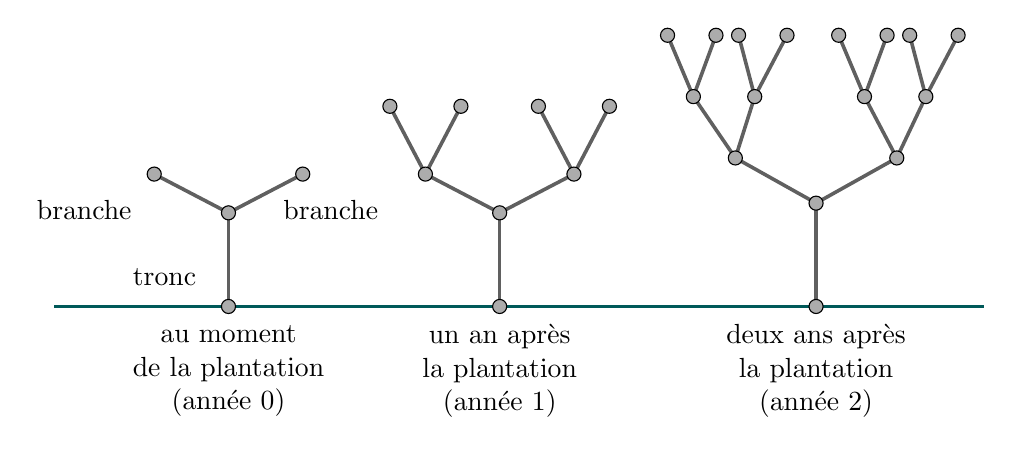
\begin{tikzpicture}[
					scale=0.82,
					point/.style={circle, draw=black, fill=gray!65, inner sep=1.8pt},
					branche/.style={line width=1.3pt, gray!75!black},
					sol/.style={line width=1.2pt, teal!70!black}
					]
					
					
					\draw[sol] (-1.7,0) -- (12.7,0);
					
					
					\coordinate (T0) at (1,0);
					\coordinate (N0) at (1,1.45);
					\coordinate (G0) at (-0.15,2.05);
					\coordinate (D0) at (2.15,2.05);
					
					\draw[branche] (T0) -- (N0);
					\draw[branche] (N0) -- (G0);
					\draw[branche] (N0) -- (D0);
					
					\node[point] at (T0) {};
					\node[point] at (N0) {};
					\node[point] at (G0) {};
					\node[point] at (D0) {};
					
					\node[left] at (-0.35,1.5) {branche};
					\node[right] at (1.7,1.5) {branche};
					\node[left] at (0.65,0.45) {tronc};
					
					\node[align=center] at (1,-1) {au moment\\de la plantation\\(année 0)};
					
					
					\coordinate (T1) at (5.2,0);
					\coordinate (N1) at (5.2,1.45);
					\coordinate (G1) at (4.05,2.05);
					\coordinate (D1) at (6.35,2.05);
					\coordinate (GG1) at (3.5,3.1);
					\coordinate (GD1) at (4.6,3.1);
					\coordinate (DG1) at (5.8,3.1);
					\coordinate (DD1) at (6.9,3.1);
					
					\draw[branche] (T1) -- (N1);
					\draw[branche] (N1) -- (G1);
					\draw[branche] (N1) -- (D1);
					\draw[branche] (G1) -- (GG1);
					\draw[branche] (G1) -- (GD1);
					\draw[branche] (D1) -- (DG1);
					\draw[branche] (D1) -- (DD1);
					
					\foreach \P in {T1,N1,G1,D1,GG1,GD1,DG1,DD1}
					{
						\node[point] at (\P) {};
					}
					
					\node[align=center] at (5.2,-1) {un an après\\la plantation\\(année 1)};
					
					
					\coordinate (T2) at (10.1,0);
					\coordinate (N2) at (10.1,1.6);
					\coordinate (G2) at (8.85,2.3);
					\coordinate (D2) at (11.35,2.3);
					\coordinate (GG2) at (8.2,3.25);
					\coordinate (GD2) at (9.15,3.25);
					\coordinate (DG2) at (10.85,3.25);
					\coordinate (DD2) at (11.8,3.25);
					\coordinate (A2) at (7.8,4.2);
					\coordinate (B2) at (8.55,4.2);
					\coordinate (C2) at (8.9,4.2);
					\coordinate (D2top) at (9.65,4.2);
					\coordinate (E2) at (10.45,4.2);
					\coordinate (F2) at (11.2,4.2);
					\coordinate (G2top) at (11.55,4.2);
					\coordinate (H2) at (12.3,4.2);
					
					\draw[branche] (T2) -- (N2);
					\draw[branche] (N2) -- (G2);
					\draw[branche] (N2) -- (D2);
					\draw[branche] (G2) -- (GG2);
					\draw[branche] (G2) -- (GD2);
					\draw[branche] (D2) -- (DG2);
					\draw[branche] (D2) -- (DD2);
					\draw[branche] (GG2) -- (A2);
					\draw[branche] (GG2) -- (B2);
					\draw[branche] (GD2) -- (C2);
					\draw[branche] (GD2) -- (D2top);
					\draw[branche] (DG2) -- (E2);
					\draw[branche] (DG2) -- (F2);
					\draw[branche] (DD2) -- (G2top);
					\draw[branche] (DD2) -- (H2);
					
					\foreach \P in {T2,N2,G2,D2,GG2,GD2,DG2,DD2,A2,B2,C2,D2top,E2,F2,G2top,H2}
					{
						\node[point] at (\P) {};
					}
					
					\node[align=center] at (10.1,-1) {deux ans après\\la plantation\\(année 2)};
					
				\end{tikzpicture}
			\end{center}
			
			Pour tout entier naturel $n$, on note $v_n$ le nombre de nouvelles branches $n$ années après la plantation. À la plantation, l'arbre possède $2$ branches, ainsi on pose $v_0=2$.
			
			\begin{enumerate}
				\item Chaque année, le nombre de nouvelles branches double.
				
				Ainsi, pour tout entier naturel $n$, on a :
				\[
				v_{n+1}=2v_n.
				\]
				
				La suite $(v_n)$ est donc une suite géométrique de raison $2$ et de premier terme $v_0=2$.
				
				On peut en déduire que, pour tout entier naturel $n$ :
				\[
				v_n=v_0\times 2^n.
				\]
				
				Donc :
				\[
				v_n=2\times 2^n=2^{n+1}.
				\]
				
				\item \begin{enumerate}
					\item Trois ans après la plantation, l'arbre possède toutes les branches déjà présentes à la plantation, ainsi que les nouvelles branches produites les années $1$, $2$ et $3$.
					
					On calcule d'abord le nombre de nouvelles branches produites chaque année :
					\[
					v_0=2,\qquad v_1=4,\qquad v_2=8,\qquad v_3=16.
					\]
					
					Le nombre total de branches trois ans après la plantation est donc :
					\begin{align*}
						v_0+v_1+v_2+v_3
						&=2+4+8+16\\
						&=30.
					\end{align*}
					
					Ainsi, trois ans après sa plantation, l'arbre possède bien $30$ branches au total.
					
					\item On considère le programme Python suivant :
					
					\begin{center}
						\fbox{\begin{minipage}{0.42\linewidth}\ttfamily
								v = 2\par
								total = 2\par
								for i in range(10):\par
								\quad v = 2 * v\par
								\quad total = total + v\par
								print(total)
						\end{minipage}}
					\end{center}
					
					Au début du programme, on a :
					\[
					v=2 \qquad \text{et} \qquad \text{total}=2.
					\]
					
					La variable $v$ représente le nombre de nouvelles branches produites pendant une année donnée.
					
					La variable $\text{total}$ représente le nombre total de branches de l'arbre depuis la plantation jusqu'à l'année considérée.
					
					La boucle \texttt{for i in range(10)} répète $10$ fois les instructions suivantes :
					\begin{itemize}[left=5mm,label={\textbullet~~}]
						\item on double la valeur de $v$ ;
						\item on ajoute cette nouvelle valeur de $v$ au total.
					\end{itemize}
					
					Après $10$ répétitions, le programme a donc ajouté les nombres :
					\[
					v_1,\ v_2,\ v_3,\ \ldots,\ v_{10}
					\]
					
					au nombre initial de branches $v_0=2$.
					
					La valeur affichée est donc :
					\begin{align*}
						v_0+v_1+v_2+\cdots+v_{10}
						&=2+4+8+\cdots+2048\\
						&=4094.
					\end{align*}
					
					Dans le contexte de l'exercice, la valeur $4\ 094$ représente donc le nombre total de branches que possède l'arbre $10$ ans après sa plantation.
				\end{enumerate}
			\end{enumerate}

\clearpage
